\section{Overview}


This tutorial demonstrates how to accommodate variation in the substitution process across sites of an alignment.
In the preceding tutorials, we assumed that all sites in an alignment evolved under an identical substitution process.
This assumption is likely to be violated biologically, since different nucleotide sites are subject to different selection pressures, such as depending on which gene or codon position the site belongs to.
Here, we will demonstrate how to specify---and select among---alternative \emph{mixed models} using \RevBayes.
This is commonly referred to as partitioned-data analysis, where two or more subsets of sites in our alignment are assumed to evolve under distinct processes.

This tutorial will construct two multi-gene models.
The first model, PS0, assumes all genes evolve under the same process parameters.
The second model, PS1, assumes all genes evolve according to the same process, but each gene has it's own set of process parameters.
The third model, PS2, partitions the data not only by gene, but also by codon position.
Each analysis will generate a {\it maximum a posteriori} tree to summarize the inferred phylogeny.
An advanced exercise introduces how to compute Bayes factors to select across various partitioning schemes.

All of the files for this analysis are provided for you and you can run these without significant effort using the \cl{source()} function in the \RevBayes console, \EG
{\tt \begin{snugshade*}
\begin{lstlisting}
source("RevBayes_scripts/model_PS0.Rev")
\end{lstlisting}
\end{snugshade*}}

If everything loaded properly, then you should see the program begin running the Markov chain Monte Carlo analysis needed for estimating the posterior distribution. If you continue to let this run, then you will see it output the states of the Markov chain once the MCMC analysis begins.

\subsection{Requirements}
We assume that you have previously completed the following tutorials:
\begin{itemize}
\item RB\_Getting\_Started
\item RB\_Data\_Tutorial
\item RB\_CTMC\_Tutorial
\item RB\_BayesFactor\_Tutorial
\end{itemize}
Accordingly, we will assume that you know how to execute and load data into \RevBayes, are familiar with some basic commands, and know how to perform Bayes factor comparisons to select among competing substitution models.



%%%%%%%%
%%   Data   %%
%%%%%%%%
\section{Data and files}

We provide several data files that we will use in this tutorial; these are the same datasets that we have used in previous tutorials.
In the \cl{data} folder, you will find the following files
\begin{itemize}
\item
\cl{primates\_cytb.nex}: Alignment of the \textit{cytochrome b} subunit from 23 primates representing 14 of the 16 families (\textit{Indriidae} and \textit{Callitrichidae} are missing).
\item
\cl{primates\_cox2.nex}: Alignment of the \textit{COX-II} gene from the same 23 primates species.
\end{itemize}



\section{Introduction}

Variation in the evolutionary process across the sites of nucleotide sequence alignments is well established, and is an increasingly pervasive feature of datasets composed of gene regions sampled from multiple loci and/or different genomes.
Inference of phylogeny from these data demands that we adequately model the underlying process heterogeneity; failure to do so can lead to biased estimates of phylogeny and other parameters \citep{Brown2007}.
%To accommodate process heterogeneity within and/or between various gene(omic) regions, we will evaluate the support for various partition schemes using Bayes factors to compare the marginal likelihoods of the candidate partition schemes.

Accounting for process heterogeneity involves adopting a `mixed-model' approach, \citep{Ronquist2003} in which the sequence alignment is first parsed into a number of partitions that are intended to capture plausible process heterogeneity within the data.
The determination of the partitioning scheme is guided by biological considerations regarding the dataset at hand.
For example, we might wish to evaluate possible variation in the evolutionary process within a single gene region (\EG between stem and loop regions of ribosomal sequences), or among gene regions in a concatenated alignment (\EG comprising multiple nuclear loci and/or gene regions sampled from different genomes).
The choice of partitioning scheme is up to the investigator and many possible partitions might be considered for a typical dataset.

%Next, a substitution model is specified for each predefined process partition (using a given model-selection criterion, such as Bayes factors).
In this exercise, we assume that each partition evolved under an independent general-time reversible model with gamma-distributed rates across sites (GTR+$\Gamma$). 
Under this model the observed data are conditionally dependent on the exchangeability rates ($\theta$), stationary base frequencies ($\pi$), and the degree of gamma-distributed among-site rate variation ($\alpha$), as well as the unrooted tree topology ($\Psi$) and branch lengths ($\nu$).
We show the graphical model representation of the GTR+$\Gamma$ mode in Figure \ref{pipeline}. 
When we assume different GTR+$\Gamma$ models for each partitions, this results in a composite model, in which all sites are assumed to share a common, unrooted tree topology and proportional branch lengths, but subsets of sites (`data partitions') are assumed to have independent substitution model parameters.
This composite model is referred to as a \emph{mixed model}. 
%\taha{need to change the graphical model above to have the same symbols as in this paragraph since this refers to the figure \ref{pipeline} and it may be harder to change that figure.}



Finally, we perform a separate MCMC simulation to approximate the joint posterior probability density of the phylogeny and other parameters.  Note that, in this approach, the mixed model is a fixed assumption of the inference (\IE the parameter estimates are conditioned on the specified mixed model), and the parameters for each process partition are independently estimated.

For most sequence alignments, several (possibly many) partition schemes of varying complexity are plausible {\it a priori}, which therefore requires a way to objectively identify the partition scheme that balances estimation bias and error variance associated with under- and over-parameterized mixed models, respectively.
Increasingly, mixed-model selection is based on \textit{Bayes factors} \citep[{\it e.g.},][]{Suchard2001}, which involves first calculating the marginal likelihood under each candidate partition scheme and then comparing the ratio of the marginal likelihoods for the set of candidate partition schemes \citep{Brandley2005,Nylander2004,Mcguire2007}.
The analysis pipeline that we will use in this tutorial is depicted in Figure \ref{pipeline}.

\begin{figure}[ht!]
\centering
\fbox{\includegraphics[width=6.8in,angle=0]{\ResourcePath figures/pipeline.eps}}
\caption{\small The analysis pipeline for Exercise 1. We will explore three partition schemes for the primates dataset.
The first model (the `uniform model', $M_0$) assumes that all sites evolved under a common GTR+$\Gamma$ substitution model.
The second model (the `moderately partitioned' model, $M_1$) invokes two data partitions corresponding to the two gene regions (cytB and cox2), and assumes each subset of sites evolved under an independent GTR+$\Gamma$ model.
The final mixed model (the `highly partitioned' model, $M_2$) invokes four data partitions---the first two partitions corresponds to the cytB gene region, where the first and second codon position sites share a partition distinct from the third codon position sites, and the cox2 has two partitions of its own, partitioned by codon positions in the same way---and each data partition is assumed evolved under an independent GTR+$\Gamma$ substitution model.
Note that we assume that all sites share a common tree topology, $\Psi$, and branch-length proportions, $\nu$, for each of the candidate partition schemes.
We perform two separate sets of analyses for each mixed model---a Metropolis-coupled MCMC simulation to approximate the joint posterior probability density of the mixed-model parameters, and a `stepping-stone' MCMC simulation to approximate the marginal likelihood for each mixed model.
The resulting marginal-likelihood estimates are then evaluated using Bayes factors to assess the fit of the data to the three candidate mixed models.  
}
\label{pipeline}
\end{figure}
\newpage



\section{Concatenated, Non-partitioned}\label{secUnif} 

Our first exercise is to construct a multi-gene analysis where all genes evolve under the same process and parameters.

To begin, load in the sequences using the \cl{readDiscreteCharacterData()} function. 
{\tt \begin{snugshade*}
\begin{lstlisting}
data_cox2 = readDiscreteCharacterData("data/primates_cox2.nex")
data_cytb = readDiscreteCharacterData("data/primates_cytb.nex")
\end{lstlisting}
\end{snugshade*}}

Since the first step in this exercise is to assume a single model across genes, we need to combine the two datasets using {\tt concatenate()}

{\tt \begin{snugshade*}
\begin{lstlisting}
data = concatenate( data_cox2, data_cytb )
\end{lstlisting}
\end{snugshade*}}

Typing \cl{data} reports the dimensions of the concatenated matrix, this provides information about the alignment:


{\tt \begin{snugshade*}
\begin{lstlisting}

   DNA character matrix with 23 taxa and 1852 characters
   =====================================================
   Origination:                   primates_cox2.nex
   Number of taxa:                23
   Number of included taxa:       23
   Number of characters:          1852
   Number of included characters: 1852
   Datatype:                      DNA

\end{lstlisting}
\end{snugshade*}}

For later use, we will store the taxon labels (\cl{names}), the number of species (\cl{n\_species}), the number of internal branches (\cl{n\_branches}), and the number of sites (\cl{n\_sites}).

{\tt \begin{snugshade*}
\begin{lstlisting}
names <- data.names()
n_species <- data.ntaxa()
n_branches <- 2 * n_species - 3
n_sites <- data.nchar()
\end{lstlisting}
\end{snugshade*}}

Additionally, we will create some move and monitor index variables to create our move and monitor vectors.

{\tt \begin{snugshade*}
\begin{lstlisting}
mvi <- 1
mni <- 1
\end{lstlisting}
\end{snugshade*}}

Now we can proceed with building our GTR$+\Gamma$ model.
First, we will define and specify a prior on the exchangeability rates of the GTR model

{\tt \begin{snugshade*}
\begin{lstlisting}
er_prior <- v(1,1,1,1,1,1) 
er ~ dnDirichlet( er_prior )
\end{lstlisting}
\end{snugshade*}}

and assign its move

{\tt \begin{snugshade*}
\begin{lstlisting}
moves[mvi++] = mvSimplexElementScale(er, alpha=10, tune=true, weight=3) 
\end{lstlisting}
\end{snugshade*}}

We can use the same type of distribution as a prior on the 4 stationary frequencies ($\pi_A, \pi_C, \pi_G, \pi_T$) since these parameters also represent proportions. 
Specify a flat Dirichlet prior density on the base frequencies:
{\tt \begin{snugshade*}
\begin{lstlisting}
pi_prior <- v(1,1,1,1) 
pi ~ dnDirichlet( pi_prior )
\end{lstlisting}
\end{snugshade*}}

The node \cl{pi} represents the $\pi$ node in Figure \ref{pipeline}.
Now add the simplex scale move on the stationary frequencies to the moves vector

{\tt \small \begin{snugshade*}
\begin{lstlisting}
moves[mvi++] = mvSimplexElementScale(pi, alpha=10, tune=true, weight=2) 
\end{lstlisting}
\end{snugshade*}}

We can finish setting up this part of the model by creating a deterministic node for the GTR rate matrix \cl{Q}. 
The \cl{fnGTR()} function takes a set of exchangeability rates and a set of base frequencies to compute the rate matrix used when calculating the likelihood of our model.
{\tt \begin{snugshade*}
\begin{lstlisting}
Q := fnGTR(er,pi)
\end{lstlisting}
\end{snugshade*}}


We will also assume that the substitution rates vary among sites according to a gamma distribution, which has two parameters: the shape parameter, $\alpha$, and the rate parameter, $\beta$. 
In order that we can interpret the branch lengths as the expected number of substitutions per site, this model assumes that the mean site rate is equal to 1.
%Consequently, we wish to specify a gamma distribution with a mean of 1.
The mean of the gamma is equal to $\alpha/\beta$, so a mean-one gamma is specified by setting the two parameters to be equal, $\alpha=\beta$.
Therefore, we need only consider the single shape parameter, $\alpha$ \citep{Yang1994a}. 
The degree of among-site substitution rate variation (ASRV) is inversely proportional to the value of the shape parameter---as the value of $\alpha$-shape parameter increases, the gamma distribution increasingly resembles a normal distribution with decreasing variance, which corresponds to decreasing levels of ASRV (Figure \ref{asrhGammaFig}).
If $\alpha = 1$, then the gamma distribution collapses to an exponential distribution with a rate parameter equal to $\beta$.
By contrast, when the value of the $\alpha$-shape parameter is $< 1$, the gamma distribution assumes a concave distribution that places most of the prior density on low rates but allows some prior mass on sites with very high rates, which corresponds to high levels of ASRV (Figure \ref{asrhGammaFig}).

\begin{figure}[h]
\centering
\fbox{\includegraphics[width=2.5in,angle=-90]{\ResourcePath figures/asrh_gamma.eps}}
\caption{\small The probability density of mean-one gamma-distributed rates under different shape parameters.}
\label{asrhGammaFig}
\end{figure}


Alternatively, we might not have good prior knowledge about the variance in site rates, thus we can place an uninformative prior on the shape parameter.
For this analysis, we will use an uniform distribution for values 0.1 to 50.0 to reflect our ignorance of what shape we expect.

Create a constant nodes called \cl{alpha\_prior\_min} and \cl{alpha\_prior\_max} to specify the interval for the uniform prior on the gamma-shape parameter
{\tt\begin{snugshade*}
\begin{lstlisting}
alpha_prior_min <- 0.1
alpha_prior_max <- 50.0
\end{lstlisting}
\end{snugshade*}}

Then create a stochastic node called \cl{alpha} to represent the $\alpha$ node in Figure \ref{pipeline}, with an exponential density as a prior:
{\tt\begin{snugshade*}
\begin{lstlisting}
alpha ~ dnUnif( alpha_prior_min, alpha_prior_max )
\end{lstlisting}
\end{snugshade*}}

The way the ASRV model is implemented involves discretizing the mean-one gamma distribution into a set number of rate categories. Thus, we can analytically marginalize over the uncertainty in the rate at each site. To do this, we need a deterministic node that is a vector of rates calculated from the gamma distribution and the number of rate categories. The \cl{fnDiscretizeGamma()} function returns this deterministic node and takes three arguments: the shape and rate of the gamma distribution and the number of categories. Since we want to discretize a mean-one gamma distribution, we can pass in \cl{alpha} for both the shape and rate.

Initialize the \cl{gamma\_rates} deterministic node vector using the  \cl{fnDiscretizeGamma()} function with \cl{4} bins:
{\tt \begin{snugshade*}
\begin{lstlisting}
norm_gamma_rates := fnDiscretizeGamma( alpha, alpha, 4, false )
\end{lstlisting}
\end{snugshade*}}

The random variable that controls the rate variation is the stochastic node \cl{alpha}. This variable is a single, real positive value (\cl{RevType = RealPos}). 
We will apply a simple scale move to this parameter.
The scale move's tuning parameter is called \cl{lambda} and this value dictates the size of the proposal.
{\tt \begin{snugshade*}
\begin{lstlisting}
moves[mvi++] = mvScale(alpha, lambda=0.1, tune=false, weight=4.0)
\end{lstlisting}
\end{snugshade*}}

Invariant sites (sites that remain fixed throughout their evolutionary history) may be seen as an extreme case of among-site rate variation.
In contrast to $+ \Gamma$ models, the $+I$ model allows site some probability of having substitution rate equal to zero.
Only if a site has an invariant pattern (they are all are equal) there is some non-zero probability of the site being classified as invariant.
(Seeing an invariant site pattern does not necessarily indicate the site evolved according to an invariant process: there is some probability of some substitution later being erased through a character reversion, which must be accounted for in the $+I$ model.)

Here, we give the probability of a site being invariant with {\tt pinvar}
{\tt \begin{snugshade*}
\begin{lstlisting}
pinvar ~ dnBeta(1,1)
moves[mvi++] = mvScale(pinvar, lambda=0.1, tune=false, weight=2.0)
moves[mvi++] = mvSlide(pinvar, delta=10.0, tune=false, weight=2.0)
\end{lstlisting}
\end{snugshade*}}

Note, if the $+\Gamma$ model allows for one rate category to take a very small value, it approximates the zero-rate value for the $+I$ model.
This means when invariant site patterns are present, the $+\Gamma$ and $+I$ models vie to explain the same underlying evolutionary process of some sites evolving at a zero or near-zero rate.

The tree topology and branch lengths are also stochastic nodes in our model. 
In Figure \ref{pipeline}, the tree topology is denoted $\Psi$ and the length of the branch leading to node $i$ is $\nu_i$.

We will assume the topology and divergence times are distributed by a birth-death process called \cl{dnBDP()} in RevBayes.
First, we will define the distribution's speciation rate, {\tt lambda}, and an extinction rate {\tt mu}

{\tt \begin{snugshade*}
\begin{lstlisting}
speciation ~ dnExponential(10.0)
extinction ~ dnExponential(10.0)
moves[mvi++] = mvScale(speciation, weight=5)
moves[mvi++] = mvScale(extinction, weight=5)
\end{lstlisting}
\end{snugshade*}}

Since we know our analysis contains only 23 of 270 known primate species, we may inform the birth-death process only a portion of taxa were sampled.
Failing to do so artificially inflates the extinction rate.

{\tt \begin{snugshade*}
\begin{lstlisting}
sampling_fraction <- 23. / 270 # 23 out of the ~ 270 primate species
\end{lstlisting}
\end{snugshade*}}

To simplify the analysis, we assume the tree height is known to be 75, although in practice this quantity should be treated as a free parameter to estimate.

{\tt \begin{snugshade*}
\begin{lstlisting}
psi ~ dnBDP(lambda=speciation, mu=extinction, rho=sampling_fraction, rootAge=75, names=names)
\end{lstlisting}
\end{snugshade*}}

Finally, we will provide moves so the MCMC may explore the space of tree topologies ({\tt mvNNI} and {\tt mvFNPR}, the nearest-neighbor interchange and fixed-node-height-prune-regraft proposals, resp.) and the space of divergence times ({\tt mvNodeTimeSlideUniform}).

{\tt \begin{snugshade*}
\begin{lstlisting}
moves[mvi++] = mvNNI(psi, weight=10.0)
moves[mvi++] = mvFNPR(psi, weight=5.0)
moves[mvi++] = mvNodeTimeSlideUniform(psi, weight=10.0)
\end{lstlisting}
\end{snugshade*}}

Also for simplicity, we assume a global molecular clock

{\tt \small \begin{snugshade*}
\begin{lstlisting}
clock ~ dnExponential(10.0)
moves[mvi++] = mvScale(clock, lambda=1, tune=true, weight=3.0)
\end{lstlisting}
\end{snugshade*}}

We now have all the parameters needed to model the phylogenetic molecular substitution process

{\tt \begin{snugshade*}
\begin{lstlisting}
phyloSeq ~ dnPhyloCTMC(tree=psi, Q=Q, branchRates=clock, siteRates=norm_gamma_rates, pInv=pinvar, type="DNA")
\end{lstlisting}
\end{snugshade*}}

To compute the likelihood, we condition the process on the data observed at the tips of the tree

{\tt \begin{snugshade*}
\begin{lstlisting}
phyloSeq.clamp(data)
\end{lstlisting}
\end{snugshade*}}

Since the model is now specified, we wrap the components in a {\tt Model} object.

{\tt \begin{snugshade*}
\begin{lstlisting}
mymodel = model(Q)
\end{lstlisting}
\end{snugshade*}}

For our MCMC analysis we need to set up a vector of \textit{monitors} to save the states of our Markov chain. 
The monitor functions are all called \cl{mn*}, where \cl{*} is the wildcard representing the monitor type.
First, we will initialize the model monitor using the \cl{mnModel} function. This creates a new monitor variable that will output the states for all model parameters when passed into a MCMC function. 
{\tt \begin{snugshade*}
\begin{lstlisting}
monitors[mni++] = mnModel(filename="output/PS0.params.txt",printgen=10)
\end{lstlisting}
\end{snugshade*}}

The \cl{mnFile} monitor will record the states for only the parameters passed in as arguments. We use this monitor to specify the output for our sampled trees and branch lengths.

{\tt \begin{snugshade*}
\begin{lstlisting}
monitors[mni++] = mnFile(psi, filename="output/PS0.tre", printgen=100)
\end{lstlisting}
\end{snugshade*}}

Finally, create a screen monitor that will report the states of specified variables to the screen with \cl{mnScreen}:
{\tt \begin{snugshade*}
\begin{lstlisting}
monitors[mni++] = mnScreen(er, pi, alpha, norm_gamma_rates, pinvar, speciation, extinction, clock, printgen=100)
\end{lstlisting}
\end{snugshade*}}

With a fully specified model, a set of monitors, and a set of moves, we can now set up the MCMC algorithm that will sample parameter values in proportion to their posterior probability. The \cl{mcmc()} function will create our MCMC object:
{\tt \begin{snugshade*}
\begin{lstlisting}
mymcmc = mcmc(mymodel, monitors, moves)
\end{lstlisting}
\end{snugshade*}}

We can run the \cl{.burnin()} member function if we wish to pre-run the chain and discard the initial states. 
{\tt \begin{snugshade*}
\begin{lstlisting}
mymcmc.burnin(generations=10000,tuningInterval=100)
\end{lstlisting}
\end{snugshade*}}


Now, run the MCMC:
{\tt \begin{snugshade*}
\begin{lstlisting}
mymcmc.run(generations=30000)
\end{lstlisting}
\end{snugshade*}}

When the analysis is complete, you will have the monitor files in your output directory.

Methods for visualizing the marginal densities of parameter values are not currently available in \RevBayes. Thus, it is important to use programs like Tracer \citep{Rambaut2011} to evaluate mixing and non-convergence. (RevBayes does, however, have a tool for convergence assessment called \cl{beca}.)

\RevBayes~can also summarize the tree samples by reading in the tree-trace file:
{\tt \begin{snugshade*}
\begin{lstlisting}
treetrace = readTreeTrace("output/PS0.tre")
treetrace.summarize()
\end{lstlisting}
\end{snugshade*}}


The \cl{mapTree()} function will summarize the tree samples and write the maximum a posteriori tree to file:
{\tt \begin{snugshade*}
\begin{lstlisting}
mapTree(treetrace,"output/PS0_map.tre")
\end{lstlisting}
\end{snugshade*}}

This completes the uniform partition analysis.
The next two sections will implement more complex partitioning schemes in a similar manner.


\section{Partitioning by Gene Region}\label{secByGene}

The uniform model used in the previous section assumes that all sites in the alignment evolved under the same process described by a shared tree, branch length proportions, and parameters of the GTR+$\Gamma$ substitution model.
However, our alignment contains two distinct gene regions---cytB and cox2---so we may wish to explore the possibility that the substitution process differs between these two gene regions.
This requires that we first specify the data partitions corresponding to these two genes, then define an independent substitution model for each data partition. 

First, we'll clear the workspace of all declared variables
{\tt \begin{snugshade*}
\begin{lstlisting}
clear()
\end{lstlisting}
\end{snugshade*}}

Since we wish to avoid individually specifying each parameterster of the GTR+$\Gamma$ model for each of our data partitions, we can \textit{loop} over our datasets and create vectors of nodes.
To do this, we begin by creating a vector of data file names:
{\tt \begin{snugshade*}
\begin{lstlisting}
filenames <- v("data/primates_cox2.nex", "data/primates_cytb.nex")
\end{lstlisting}
\end{snugshade*}}

Set a variable for the number of partitions:
{\tt \begin{snugshade*}
\begin{lstlisting}
n_parts <- filenames.size()
\end{lstlisting}
\end{snugshade*}}

And create a vector of data matrices called \cl{data}:
{\tt \begin{snugshade*}
\begin{lstlisting}
for (i in 1:n_parts){
   data[i] = readDiscreteCharacterData(filenames[i])
}
\end{lstlisting}
\end{snugshade*}}

Next, we can initialize some important variables. This does require, however, that both of our alignments have the same number of species and matching tip names.
{\tt \begin{snugshade*}
\begin{lstlisting}
n_species <- data[1].ntaxa()
names <- data[1].names()
n_branches <- 2 * n_species - 3
\end{lstlisting}
\end{snugshade*}}

{\tt \begin{snugshade*}
\begin{lstlisting}
mvi <- 1
mni <- 1
\end{lstlisting}
\end{snugshade*}}


\subsection{Specify the Parameters by Looping Over Partitions}

We can avoid creating unique names for every node in our model if we use a \cl{for} loop to iterate over our partitions. Thus, we will only have to type in our entire GTR+$\Gamma$ model parameters once. 
This will produce a vector for each of the unlinked parameters --- e.g., there will be a vector of \cl{alpha} nodes where the stochastic node for the first partition (cytB) will be \cl{alpha[1]} and the stochastic node for the second partition (cox2) will be called \cl{alpha[2]}.

The script for the model, {\tt RevBayes\_scripts/model\_PS1.Rev}, creates the model parameters for each partition in one large loop.
Here, we will split the loop into smaller parts to achieve the same end.

First, we will create the GTR rate matrix for partition $i$ by first creating exchangeability rates
{\tt \small \begin{snugshade*}
\begin{lstlisting}
for (i in 1:n_parts) {
  er_prior[i] <- v(1,1,1,1,1,1)
  er[i] ~ dnDirichlet(er_prior[i])
  moves[mvi++] = mvSimplexElementScale(er[i], alpha=10, tune=true, weight=3) 
}
\end{lstlisting}
\end{snugshade*}}

and stationary frequencies

{\tt \small \begin{snugshade*}
\begin{lstlisting}
for (i in 1:n_parts) {
  pi_prior[i] <- v(1,1,1,1)
  pi[i] ~ dnDirichlet(pi_prior[i])
  moves[mvi++] = mvSimplexElementScale(pi[i], alpha=10, tune=true, weight=2)
}
\end{lstlisting}
\end{snugshade*}}

then passing those parameters into a rate matrix function

{\tt \small \begin{snugshade*}
\begin{lstlisting}
for (i in 1:n_parts) {
  Q[i] := fnGTR(er[i],pi[i]) 
}
\end{lstlisting}
\end{snugshade*}}

which states the rate matrix ({\tt Q[i]}) for partition $i$ is determined by the exchangeability rates ({\tt er[i]}) and stationary frequencies ({\tt pi[i]}) also defined for partition $i$.
Following this format, we construct the remainin partition parameters: the $+\Gamma$ mixture model

{\tt \small \begin{snugshade*}
\begin{lstlisting}
for (i in 1:n_parts) {
  alpha_prior_min[i] <- 0.1
  alpha_prior_max[i] <- 50.0
  alpha[i] ~ dnUnif( alpha_prior_min[i], alpha_prior_max[i] )
  norm_gamma_rates[i] := fnDiscretizeGamma( alpha[i], alpha[i], 4, false )
  moves[mvi++] = mvScale(alpha[i], lambda=0.8, tune=true, weight=3.0)
}
\end{lstlisting}
\end{snugshade*}}

the $+I$ invariant sites model

{\tt \small \begin{snugshade*}
\begin{lstlisting}
for (i in 1:n_parts) {
  pinvar[i] ~ dnBeta(1,1)
  moves[mvi++] = mvScale(pinvar[i], lambda=0.1, tune=true, weight=2.0)
  moves[mvi++] = mvSlide(pinvar[i], delta=0.1, tune=true, weight=2.0)
}
\end{lstlisting}
\end{snugshade*}}

and the per-partition molecular clock

{\tt \small \begin{snugshade*}
\begin{lstlisting}
for (i in 1:n_parts) {
  part_rate_mult[i] ~ dnExponential( 1.0 )
  moves[mvi++] = mvScale(part_rate_mult[i], lambda=1.0, tune=true, weight=2.0)
}
\end{lstlisting}
\end{snugshade*}}

Our two genes evolve under different GTR rate matrices with different mean-one gamma distributions on the site rates.
However, we do assume that they share a single topology and set of branch lengths.
{\tt \begin{snugshade*}
\begin{lstlisting}
speciation ~ dnExponential(10.)
extinction ~ dnExponential(10.)

# rescaling mv on speciation and extinction rates
moves[mvi++] = mvScale(speciation, lambda=1, tune=true, weight=3.0)
moves[mvi++] = mvScale(extinction, lambda=1, tune=true, weight=3.0)

sampling_fraction <- 23. / 270 # 23 out of the ~ 270 primate species

psi ~ dnBDP(lambda=speciation, mu=extinction, rho=sampling_fraction, rootAge=75, names=names)

# moves on the tree
moves[mvi++] = mvNNI(psi, weight=10.0)
moves[mvi++] = mvFNPR(psi, weight=5.0)
moves[mvi++] = mvNodeTimeSlideUniform(psi, weight=10.0)
\end{lstlisting}
\end{snugshade*}}

which is the same as was specified for {\tt model\_PS0.Rev}.

Since we have a rate matrix and a site-rate model for each partition, we must create a phylogenetic CTMC for each gene. 
Additionally, we must fix the values of these nodes by attaching their respective data matrices.
These two nodes are linked by the \cl{psi} node and their log-likelihoods are added to get the likelihood of the whole DAG.
{\tt \begin{snugshade*}
\begin{lstlisting}
for (i in 1:n_parts) {
  phyloSeq[i] ~ dnPhyloCTMC(tree=psi, Q=Q[i], branchRates=part_rate_mult[i], siteRates=norm_gamma_rates[i], pInv=pinvar[i], type="DNA")
  phyloSeq[i].clamp(data[i])
}
\end{lstlisting}
\end{snugshade*}}

The remaining steps should be familiar:
wrap the model components in a model object

{\tt \begin{snugshade*}
\begin{lstlisting}
mymodel = model(psi)
\end{lstlisting}
\end{snugshade*}}

create the monitors

{\tt \begin{snugshade*}
\begin{lstlisting}
monitors[mni++] = mnScreen(er, pi, alpha, norm_gamma_rates, pinvar, speciation, extinction, part_rate_mult, printgen=100)
monitors[mni++] = mnFile(psi, filename="output/PS1.tre", printgen=100)
monitors[mni++] = mnFile(er[1], pi[1], alpha[1], norm_gamma_rates[1], pinvar[1], part_rate_mult[1], er[2], pi[2], alpha[2], norm_gamma_rates[2], pinvar[2], part_rate_mult[2], speciation, extinction, filename="output/PS1.params.txt",printgen=10)
\end{lstlisting}
\end{snugshade*}}

configure and run the MCMC analysis

{\tt \begin{snugshade*}
\begin{lstlisting}
mymcmc = mcmc(mymodel, moves, monitors)
mymcmc.burnin(10000,100)
mymcmc.run(30000)
\end{lstlisting}
\end{snugshade*}}

and summarize the posterior density of trees with a MAP tree

{\tt \begin{snugshade*}
\begin{lstlisting}
treetrace = readTreeTrace("output/PS1.tre")
treetrace.summarize()
mapTree(treetrace,"output/PS1_map.tre")
\end{lstlisting}
\end{snugshade*}}



\section{Partitioning by Codon Position and by Gene}\label{secExtremeP}

Because of the genetic code, we often find that different positions within a codon (first, second, and third) evolve at different rates.
Thus, using our knowledge of biological data, we can devise a third approach that further partitions our alignment. 
For this exercise, we will partition sites within the cytB and cox2 gene by codon position.

{\tt \begin{snugshade*}
\begin{lstlisting}
clear()
data_cox2 <- readDiscreteCharacterData("data/primates_cox2.nex")
data_cytb <- readDiscreteCharacterData("data/primates_cytb.nex")
\end{lstlisting}
\end{snugshade*}}

We must now add our codon-partitions to the \cl{data} vector.
The first and second elements in the {\tt data} vector will describe cytB data, and the third and fourth elements will describe cox2 data.
Moreover, the first and third elements will describe the evolutionary process for the first and second codon position sites, while the second and fourth elements describe the process for the third codon position sites alone.

We can create this by calling the helper function \cl{setCodonPartition()}, which is a member function of the data matrix. 
We are assuming that the gene is \textit{in frame}, meaning the first column in your alignment is a first codon position. 
The \cl{setCodonPartition()} function takes a single argument, the position of the alignment you wish to extract. 
It then returns every third column, starting at the index provided as an argument.

Before we can use the use the \cl{setCodonPartition()} function, we must first populate the position in the \cl{data} matrix with some sequences. 
Then we call the member function of \cl{data[1]} to exclude all but the 1$^{st}$ and 2$^{nd}$ positions for cox2.
{\tt \begin{snugshade*}
\begin{lstlisting}
data[1] <- data_cox2
data[1].setCodonPartition( v(1,2) )
\end{lstlisting}
\end{snugshade*}}

Assign the 3$^{rd}$ codon positions for cox2 to \cl{data[2]}:
{\tt \begin{snugshade*}
\begin{lstlisting}
data[2] <- data_cox2
data[2].setCodonPartition( 3 )
\end{lstlisting}
\end{snugshade*}}

Then repeat for cytB, being careful to store the subsetted data to elements 3 and 4:
{\tt \begin{snugshade*}
\begin{lstlisting}
data[3] <- data_cytb
data[3].setCodonPartition( v(1,2) )
data[4] <- data_cytb
data[4].setCodonPartition( 3 )
\end{lstlisting}
\end{snugshade*}}

Now we can query the vector of data matrices to get the size, which is 4:
{\tt \begin{snugshade*}
\begin{lstlisting}
n_parts <- data.size()
\end{lstlisting}
\end{snugshade*}}

Record the number of sites per partition:
{\tt \begin{snugshade*}
\begin{lstlisting}
for (i in 1:n_parts)
    n_sites[i] <- data[i].nchar()
\end{lstlisting}
\end{snugshade*}}

And set the special variables from the data:
{\tt \begin{snugshade*}
\begin{lstlisting}
n_species <- data[1].ntaxa()
names <- data[1].names()
n_branches <- 2 * n_species - 3
\end{lstlisting}
\end{snugshade*}}

Create index variables to populate the move and monitor vectors.
{\tt \begin{snugshade*}
\begin{lstlisting}
mvi <- 1
mni <- 1
\end{lstlisting}
\end{snugshade*}}

Setting up the GTR+$\Gamma$ model is just like in the two-gene analysis, except this time \cl{n\_parts} is equal to 4, so now our vectors of stochastic nodes should all contain nodes for the four pairs of codon-gene partitions.

The script for the model, {\tt RevBayes\_scripts/model\_PS2.Rev}, creates the model parameters for each partition in one large loop.
Like before, we will split the loop into smaller parts to achieve the same end.

First, we will create the GTR rate matrix for partition $i$ by first creating exchangeability rates
{\tt \small \begin{snugshade*}
\begin{lstlisting}
for (i in 1:n_parts) {
  er_prior[i] <- v(1,1,1,1,1,1)
  er[i] ~ dnDirichlet(er_prior[i])
  moves[mvi++] = mvSimplexElementScale(er[i], alpha=10, tune=true, weight=3) 
}
\end{lstlisting}
\end{snugshade*}}

and stationary frequencies

{\tt \small \begin{snugshade*}
\begin{lstlisting}
for (i in 1:n_parts) {
  pi_prior[i] <- v(1,1,1,1)
  pi[i] ~ dnDirichlet(pi_prior[i])
  moves[mvi++] = mvSimplexElementScale(pi[i], alpha=10, tune=true, weight=2)
}
\end{lstlisting}
\end{snugshade*}}

then passing those parameters into a rate matrix function

{\tt \small \begin{snugshade*}
\begin{lstlisting}
for (i in 1:n_parts) {
  Q[i] := fnGTR(er[i],pi[i]) 
}
\end{lstlisting}
\end{snugshade*}}

which states the rate matrix ({\tt Q[i]}) for partition $i$ is determined by the exchangeability rates ({\tt er[i]}) and stationary frequencies ({\tt pi[i]}) also defined for partition $i$.
Following this format, we construct the remainin partition parameters: the $+\Gamma$ mixture model

{\tt \small \begin{snugshade*}
\begin{lstlisting}
for (i in 1:n_parts) {
  alpha_prior_min[i] <- 0.1
  alpha_prior_max[i] <- 50.0
  alpha[i] ~ dnUnif( alpha_prior_min[i], alpha_prior_max[i] )
  norm_gamma_rates[i] := fnDiscretizeGamma( alpha[i], alpha[i], 4, false )
  moves[mvi++] = mvScale(alpha[i], lambda=0.8, tune=true, weight=3.0)
}
\end{lstlisting}
\end{snugshade*}}

the $+I$ invariant sites model

{\tt \small \begin{snugshade*}
\begin{lstlisting}
for (i in 1:n_parts) {
  pinvar[i] ~ dnBeta(1,1)
  moves[mvi++] = mvScale(pinvar[i], lambda=0.1, tune=true, weight=2.0)
  moves[mvi++] = mvSlide(pinvar[i], delta=0.1, tune=true, weight=2.0)
}
\end{lstlisting}
\end{snugshade*}}

and the per-partition molecular clock

{\tt \small \begin{snugshade*}
\begin{lstlisting}
for (i in 1:n_parts) {
  part_rate_mult[i] ~ dnExponential( 1.0 )
  moves[mvi++] = mvScale(part_rate_mult[i], lambda=1.0, tune=true, weight=2.0)
}
\end{lstlisting}
\end{snugshade*}}


Note that applying the per-partition model parameters only depends on the number of partitions, which means the script describing the partitioned model will work so long as you correctly populate the {\tt data} vector.

We are still assuming that the genes share a single topology and branch lengths.
{\tt \begin{snugshade*}
\begin{lstlisting}
speciation ~ dnExponential(10.)
extinction ~ dnExponential(10.)

# rescaling mv on speciation and extinction rates
moves[mvi++] = mvScale(speciation, lambda=1, tune=true, weight=3.0)
moves[mvi++] = mvScale(extinction, lambda=1, tune=true, weight=3.0)

sampling_fraction <- 23. / 270 # 23 out of the ~ 270 primate species

psi ~ dnBDP(lambda=speciation, mu=extinction, rho=sampling_fraction, rootAge=75, names=names)

# moves on the tree
moves[mvi++] = mvNNI(psi, weight=10.0)
moves[mvi++] = mvFNPR(psi, weight=5.0)
moves[mvi++] = mvNodeTimeSlideUniform(psi, weight=10.0)
\end{lstlisting}
\end{snugshade*}}

We must specify a phylogenetic CTMC node for each of our partition models.
{\tt \begin{snugshade*}
\begin{lstlisting}
for (i in 1:n_parts){
  phyloSeq[i] ~ dnPhyloCTMC(tree=psi, Q=Q[i], branchRates=part_rate_mult[i], siteRates=norm_gamma_rates[i], pInv=pinvar[i], type="DNA")
  phyloSeq[i].clamp(data[i])
}

\end{lstlisting}
\end{snugshade*}}

And then wrap up the DAG using the \cl{model()} function:
{\tt \begin{snugshade*}
\begin{lstlisting}
mymodel = model(psi)
\end{lstlisting}
\end{snugshade*}}

Monitor the model parameters, monitoring the tree seperately:

{\tt \begin{snugshade*}
\begin{lstlisting}
monitors[mni++] = mnScreen(er, pi, alpha, norm_gamma_rates, pinvar, speciation, extinction, part_rate_mult, printgen=100)
monitors[mni++] = mnFile(psi, filename="output/PS2.tre", printgen=100)
monitors[mni++] = mnFile(er[1], pi[1], alpha[1], norm_gamma_rates[1], pinvar[1], part_rate_mult[1], er[2], pi[2], alpha[2], norm_gamma_rates[2], pinvar[2], part_rate_mult[2], er[3], pi[3], alpha[3], norm_gamma_rates[3], pinvar[3], part_rate_mult[3], er[4], pi[4], alpha[4], norm_gamma_rates[4], pinvar[4], part_rate_mult[4], speciation, extinction, filename="output/PS2.params.txt",printgen=10)
\end{lstlisting}
\end{snugshade*}}

Set up and run the MCMC analysis:

{\tt \begin{snugshade*}
\begin{lstlisting}
mymcmc = mcmc(mymodel, moves, monitors)
mymcmc.burnin(10000,100)
mymcmc.run(100000) # run for fewer iterations for classroom exercises
\end{lstlisting}
\end{snugshade*}}

And, when MCMC completes, compute the MAP tree:

{\tt \begin{snugshade*}
\begin{lstlisting}
treetrace = readTreeTrace("output/PS2.tre")
treetrace.summarize()
mapTree(treetrace,"output/PS2_map.tre")
\end{lstlisting}
\end{snugshade*}}

\subsection{Exercises}
\begin{itemize}

\item {\bf 1) Reviewing posterior estimates.} Open the {\tt PS2.params.txt} file in Tracer. Remember that partitions 1 and 2 are for cox2, partitions 3 and 4 are for cytB, partitions 1 and 3 are for sites in the first and second codon positions (per gene), and partitions 2 and 4 are for sites in the third and fourth codon positions (per gene).

Aside from the tree topology and divergence times, each partition is modeled to have its own set of parameters.
However, the posterior estimates for some parameters appear quite similar between some pairs of partitions yet different between other pairs of partitions.
For example, {\tt part\_rate\_mult} is the per-partition molecular clock.
This clock is approximately two orders of magnitude faster for partitions 2 and 4 (third codon position sites) than it is for partitions 1 and 3 (non-third codon position sites).

Identify other parameter-partition relationships like this in the posterior.
Under this model, would you consider the gene or the codon site position to hold greater influence over the site's evolutionary mode?

\item {\bf 2) Comparison of MAP trees.} Open the three inferred MAP trees in FigTree.
Check to enable ``Node Labels'', click ``Display'' and select ``posterior'' from the dropdown menu.
Internal nodes now report the probability of the clade appearing in the posterior density of sampled trees.
Do different models yield different tree topologies?
Generally, do complex models provide higher or lower clade support?

\item {\bf 3) Partitioned model selection.}
Bayes factors are computed as the ratio of marginal likelihoods (see the marginal likelihood tutorial (Section XXX) for more details).
Rather than constructing the analysis with an {\tt mcmc} object, marginal likelihood computations rely on output from a {\tt powerPosterior} object.

Copy {\tt model\_PS0.Rev} to {\tt marginal\_PS0.Rev}.
In {\tt marginal\_PS0.Rev}, delete all lines after the {\tt model} function is called, so the MCMC is never run and the MAP tree is never computed.
Additionally, remove the line creating {\tt mnScreen}, which will conflict with output produced by the power posterior analysis.



Instead, configure and run a power posterior analysis

{\tt \begin{snugshade*}
\begin{lstlisting}
pow_p = powerPosterior(mymodel, moves, monitors, "output/model1.out", cats=50)
pow_p.burnin(generations=10000,tuningInterval=1000)
pow_p.run(generations=1000)
\end{lstlisting}
\end{snugshade*}}

then compute the marginal likelihood using the stepping stone sampler

{\tt \begin{snugshade*}
\begin{lstlisting}
ss = steppingStoneSampler(file="output/PS0.out", powerColumnName="power", likelihoodColumnName="likelihood")
ss.marginal()
\end{lstlisting}
\end{snugshade*}}

and again using the path sampler

{\tt \begin{snugshade*}
\begin{lstlisting}
ps = pathSampler(file="PS0.out", powerColumnName="power", likelihoodColumnName="likelihood")
ps.marginal()\end{lstlisting}
\end{snugshade*}}


\item {\bf 4) Customized partition models (advanced).} Create the partitioned model where first, second, and third codon positions are partitioned per gene.
The substitution parameters for each partition are independent {\it except} the first and second codon positions per gene share stationary frequencies.
These parameters would be $\pi_{12}^{(cytB)}$, $\pi_{3}^{(cytB)}$, $\pi_{12}^{(cox2)}$, $\pi_{3}^{(cox2)}$.

The easiest way to accomplish this is to copy {\tt model\_PS2.Rev} to {\tt model\_PS3.Rev} and modify the new file's contents.
Specifically, you will need to adjust how the codon position partitions are defined to yield six (instead of four) partitions.
When looping over partitions, you will need an if-statement to assign stationary frequencies properly.
Take some care when applying monitors and moves to the new model.


\end{itemize}

\bibliographystyle{sysbio}
\bibliography{\ResourcePath refs}
